\documentclass[a4paper]{article}

\usepackage[]{algorithm2e}
\usepackage{amsmath}
\usepackage{graphicx}
\usepackage{hyperref}

\SetKw{Wait}{wait}
\SetKwBlock{Loop}{loop}{end}
\SetKwFunction{Sample}{sample}
\SetKwFunction{CreateProcess}{createProcess}
\SetKwFunction{DeleteProcess}{deleteProcess}
\SetKwFunction{CreateHost}{createHost}
\SetKwFunction{DeleteHost}{deleteHost}
\SetKwFunction{CreateFlow}{createFlow}
\SetKwProg{Process}{process}{}{}
\SetKwFunction{Main}{main}
\SetKwFunction{Agent}{agent}
\SetKwFunction{Mobility}{mobility}

\title{Campus Bundle}
\author{}
\date{}

\begin{document}
\maketitle

All parameters are listed in Figure \ref{fig:params}. Topology information is derived from \url{../docs/cisco-campus-guidelines.pdf}. Specifically Pages 12 and 13 are of 
intereset which depict a recommended two- and three-tier topology. Algorithm \ref{alg:traffic} shows the Traffic Process which is executed alongside the simulation.

\begin{figure}
\begin{tabular}{llll}
Parameter & Type & Value & Info\\
Load & extrinsic & - &
Alter Session Arrival\\
Distribution-Layer Size & extrinsic & - & \\
Access-Layer Size & extrinsic & - & \\
Session Arrival & intrinsic & Figure \ref{fig:dists} Row 1 & \\
AP Selection & intrinsic & Figure \ref{fig:dists} Row 2 & \\
Flow Interarrival & intrinsic & Figure \ref{fig:dists} Row 3 & \\
Flow Number & intrinsic & Figure \ref{fig:dists} Row 4 & \\
Flow Size & intrinsic & Figure \ref{fig:dists} Row 5 & \\
Flow Destination & intrinsic & 80/20 Rule
\end{tabular}
\caption{Intrinsic and Extrinsic Parameters}
\label{fig:params}
\end{figure}

\begin{figure}
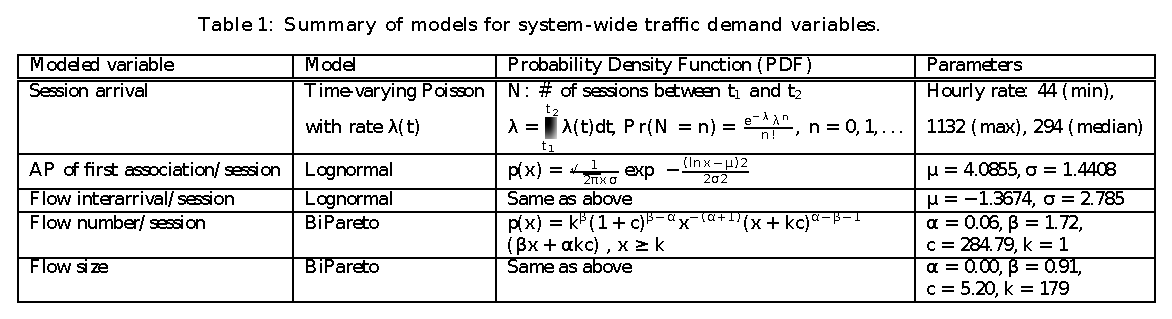
\includegraphics[width=\textwidth]{../docs/parameters-1}
\caption{Distributions}
\label{fig:dists}
\end{figure}

\begin{algorithm}[H]
\Process{\Main{}}{
\Loop{
$\CreateProcess{\Agent}$; \tcp{create agent process}
\Wait \Sample{1}; \tcp{wait for next agent}
}
}
\Process{\Agent{}}{
$AP \gets \Sample{2}$; \tcp{select random access point}
$V \gets \texttt{random point in voronoi region of } AP$\;
$H \gets \CreateHost{V}$\;
$P \gets \CreateProcess{\Mobility, H}$; \tcp{create mobility process}
\For{i $\gets$ 1 \KwTo \Sample{4}}{
$S \gets \Sample{5}$; \tcp{select random flow size}
$\CreateFlow{H, 100, D, S}$\;
\Wait \Sample{3}; \tcp{wait for next flow}
}
\DeleteProcess{P}\;
\DeleteHost{H}\;
}
\Process{\Mobility{H}}{
\Loop{
$OAP \gets \Sample{2}$; \tcp{select random access point}
$OV \gets \texttt{random point in voronoi region of } OAP$\;
\While{not at OV}{
$\texttt{step along path to } OV$\;
\Wait 1s\;
}
\Wait \texttt{random time}\;
}
}
\caption{Traffic Process}
\label{alg:traffic}
\end{algorithm}
\end{document}
